\documentclass[times, utf8, seminar]{fit}


%\batchmode
%\usepackage{booktabs}
\usepackage{listings}
\usepackage{longtable}
\usepackage{xcolor}
\usepackage{float}
\usepackage{enumitem}
\usepackage{hyperref}
\usepackage{enumerate}
\usepackage{graphicx}
\usepackage{etoolbox}
\usepackage{datetime}
\usepackage{needspace}
\usepackage[compact]{titlesec}
\usepackage{verbatim}
%\usepackage{hyperref}
%\titleformat{\chapter}[display]{\normalfont\huge\bfseries}{\chaptertitlename\ \thechapter}{20pt}{\Huge}


%http://stackoverflow.com/questions/3279194/remove-spacing-before-chapter-in-latex
%\usepackage{titlesec}
%\titleformat{\chapter}[display]
%{\normalfont\huge\bfseries}{\chaptertitlename\ \thechapter}{20pt}{\Huge}
% this alters "before" spacing (the second length argument) to 0
%\titlespacing*{\chapter}{0pt}{-20pt}{40pt}

%\renewcommand*{\chapterheadstartvskip}{\vspace*{0.5cm}}
%\renewcommand*{\chapterheadendvskip}{\vspace{1cm}}

% http://tex.stackexchange.com/questions/40436/vertical-space-before-section-title-with-titlesec

%\usepackage[compact]{titlesec}
\usepackage{setspace}
\onehalfspacing

%\titleformat{\section}{\normalfont\bfseries}{\thesection}{1em}{}
%\titlespacing{\section}{0pt}{0pt}{0pt}

\begin{document}
\widowpenalty=300
\clubpenalty=300

\lstset{
  language=bash,
  backgroundcolor=\color{gray!25},
  basicstyle=\ttfamily \footnotesize,
  breaklines=true,
  prebreak=\raisebox{0ex}[0ex][0ex] \hookleftarrow,
  columns=fullflexible
}


\title{Agilni \emph{software development},\newline test \& deployment}

\author{Ernad Husremović}
\brindex{DL 2792}
\verzija {0.0.5}

\mentor{mr. Adil Joldić}

\maketitle

\tableofcontents

%\listoftables
%\listoffigures
\newpage

\begin{abstract}

U ovom radu se na bazi konkretnog primjera\footnote{"HOWTO" stil} prezentuje infrastruktura za testiranje i instalaciju u produkcijskom okruženju (''test'' \& ''deploy'' infrastructure). Obradićemo instalaciju ''Gitlab'' servera koristeći sljedeće tehnologije i servise:
\begin{enumerate}
  \item Github/git \url{https://github.com/hernad/gitlabhq}
  \item Vagrant  \url{http://vagrantup.com/}
  \item Chef opscode \url{http://www.opscode.com/chef}
  \item Rackspace cloud \url{http://www.rackspace.com/cloud}
\end{enumerate}

\keywords{open source software, OSS, chef, vagrant, rackspace, git, github}
\end{abstract}

% abstract end

\chapter{Uvod}

%\vspace*{-1.2cm}
\section{Gitlab}
Gitlab je web servis koji obezbjeđuje upravljanje softverskim projektima. Gitlab obezbjeđuje sljedeće funkcije:
\begin{enumerate}
  \item Git source code management - hostiranje git repozitorija
  \item Issue management - elektronsko praćenje aktivnosti developera
  \item Milestone management - pojedine aktivnosti (issues) se mogu vezati uz odgovarajuću verziju (iteraciju) - ''milestone''
  \item Code snippets (code templates) - publikovanje uzoraka izvornog koda koje će tim koristiti
  \item Code/Commit review - komentarisanje izvornog koda
  \item Wikies - wikiji omogućavaju timski razvoj projektne dokumentacije
\end{enumerate}

\section{Gitlab arhitektura}
''Gitlab'' je složen softverski sistem sastaljen od sljedećih komponenti:
\begin{enumerate}
  \item ubuntu linux server
  \item ''ruby on rails'' framework je korišten za izradu web front-end-a.
  \item ''resque'' za background jobs \url{https://github.com/defunkt/resque}
  \item ''redis'' nosql (koristi ga ''resque'')
  \item ''mysql'' database backend\footnote{može se koristiti i postgresql}
  \item ''gitolite'' za upravljanje git repozitorijima
\end{enumerate}


\chapter{Gitlab merge from upstream}

\setlength{\parindent 0cm}
gitlabhq\$ \verb+git fetch gitlabhq+
\begin{lstlisting}
remote: Counting objects: 570, done.
remote: Compressing objects: 100\% (174/174), done.
remote: Total 342 (delta 262), reused 237 (delta 165)
Receiving objects: 100\% (342/342), 43.70 KiB, done.
Resolving deltas: 100\% (262/262), completed with 122 local objects.
From git://github.com/gitlabhq/gitlabhq
   dd4d124..3c7806c  master     -> gitlabhq/master
\end{lstlisting}


gitlabhq\$ \verb+git branch -l+
\begin{lstlisting}
* master
\end{lstlisting}


gitlabhq\$ \verb+git commit -a+
\begin{lstlisting}
[master 9bacff4] http://www.quora.com/Ruby-on-Rails/What-is-schema-rb-in-rails-project
 1 file changed, 19 insertions(+), 19 deletions(-)
\end{lstlisting}



gitlabhq\$ \verb+git diff HEAD^1 HEAD+
\begin{lstlisting}
diff --git a/db/schema.rb b/db/schema.rb
index 51ab207..19eb8eb 100644
--- a/db/schema.rb
+++ b/db/schema.rb
@@ -69,8 +69,8 @@ ActiveRecord::Schema.define(:version => 20121026114600) do
     t.boolean  "closed",                              :default => false, :null => false
     t.datetime "created_at",                                             :null => false
     t.datetime "updated_at",                                             :null => false
-    t.text     "st_commits",    :limit => 2147483647
-    t.text     "st_diffs",      :limit => 2147483647
+    t.text     "st_commits",    :limit => 4294967295

  ...

     t.integer  "project_id"
     t.string   "attachment"
     t.string   "line_code"
@@ -156,30 +156,30 @@ ActiveRecord::Schema.define(:version => 20121026114600) do
   end
 
   create_table "users", :force => true do |t|
\end{lstlisting}


gitlabhq\$ git merge gitlabhq/master

\begin{lstlisting}
Removing lib/gitlab/encode.rb
Removing gitlab
Auto-merging doc/development.md
Removing Procfile.production
Merge made by the recursive strategy
 .travis.yml                                        |    2 +-
 CHANGELOG                                          |    2 +-
 Gemfile                                            |    4 +-
 Gemfile.lock                                       |   12 +++-
 Procfile.production                                |    2 -
 VERSION                                            |    2 +-
 app/assets/images/event_filter_comments.png        |  Bin 0 -> 750 bytes
 app/assets/images/event_filter_merged.png          |  Bin 0 -> 463 bytes
 app/assets/images/event_filter_push.png            |  Bin 0 -> 632 bytes
 
 ...

 app/controllers/application_controller.rb          |    9 +++
 app/controllers/blob_controller.rb                 |   10 +--
 app/controllers/dashboard_controller.rb            |   11 ++-
 app/controllers/profile_controller.rb              |    2 +-

 ...

 app/views/blame/show.html.haml                     |    4 +-
 app/views/commits/_commit.html.haml                |    4 +-
 app/views/commits/_head.html.haml                  |    5 ++
 app/views/dashboard/index.html.haml                |    9 ++-
 
 ... 
 
 delete mode 100644 Procfile.production
 create mode 100644 app/assets/images/event_filter_comments.png
 create mode 100644 app/assets/images/event_filter_merged.png
 create mode 100644 app/assets/images/event_filter_push.png
 ...
 delete mode 100644 lib/gitlab/encode.rb
 create mode 100644 lib/gitlab/git_stats.rb
 create mode 100644 vendor/assets/javascripts/g.bar-min.js
 create mode 100644 vendor/assets/javascripts/g.raphael-min.js
\end{lstlisting}



gitlabhq\$ git push origin master

\begin{lstlisting}
Counting objects: 581, done.
Delta compression using up to 8 threads.
Compressing objects: 100\% (85/85), done.
Writing objects: 100\% (350/350), 45.00 KiB, done.
Total 350 (delta 267), reused 342 (delta 262)
To git@github.com:hernad/gitlabhq.git
   038ac96..28f5807  master -> master

\end{lstlisting}

\begin{figure}[H]
\centering
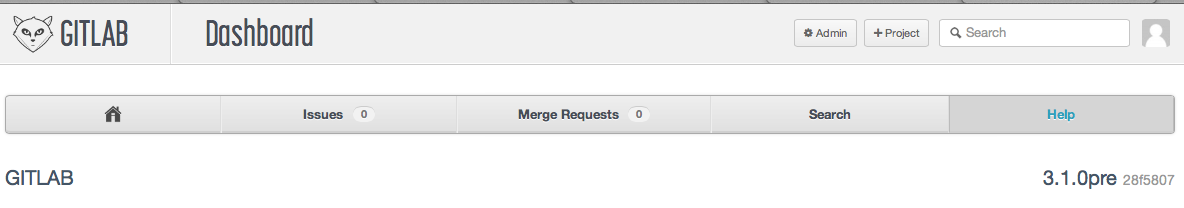
\includegraphics[width=15cm]{img/gitlab_hernad_310_after_merge.png}
\caption{Gitlabhq nakon `merge' operacije sa `upstream' projektom}
\end{figure}

\begin{figure}[H]
\centering
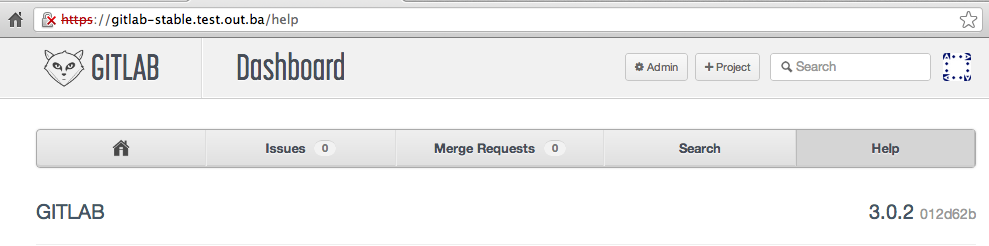
\includegraphics[width=15cm]{img/gitlab_stable_3.0.2.png}
\caption{Gitlabhq - stable 3.0.2}
\end{figure}


\begin{figure}[H]
\centering
\includegraphics[width=15cm]{img/gitlabhq_3.0.3.png}
\caption{Gitlabhq - 3.0.3}
\end{figure}


\chapter{Instalacija gitlab-a na rackspacecloud server}

\begin{lstlisting}

Server sa imenom gitlab.knowhow.out.ba vec postoji !
Server: gitlab.knowhow.out.ba IP: 198.101.149.48
server je kreiran !
Server: gitlab.knowhow.out.ba IP: 198.101.149.48
vrsim update domena knowhow.out.ba, zapis gitlab.knowhow.out.ba sa javnom adresom 198.101.149.48
./manage_domains.py -d knowhow.out.ba -r gitlab.knowhow.out.ba -i 198.101.149.48
dns_domain: knowhow.out.ba dns_record: gitlab.knowhow.out.ba ip_address 198.101.149.48

....

[2012-11-12T11:15:43+00:00] INFO: template[/etc/rvmrc] mode changed to 644
[2012-11-12T11:15:43+00:00] INFO: Processing execute[install system-wide RVM] action run (rvm::system_install line 76)
[2012-11-12T11:15:43+00:00] INFO: Processing execute[upgrade system-wide RVM to none] action run (rvm::system_install line 110)
[2012-11-12T11:15:43+00:00] INFO: Processing rvm_ruby[ruby-1.9.3-p327] action install (rvm::system line 170)
/root/vagrant_gitlab/cookbooks/rvm/libraries/rvm_chef_user_environment.rb:36: warning: class variable access from toplevel
[2012-11-12T11:15:45+00:00] INFO: Processing package[build-essential] action install (/root/vagrant_gitlab/cookbooks/rvm/providers/ruby.rb line 156)
[2012-11-12T11:15:45+00:00] INFO: Processing package[openssl] action install (/root/vagrant_gitlab/cookbooks/rvm/providers/ruby.rb line 156)
[2012-11-12T11:15:45+00:00] INFO: Processing package[libreadline6] action install (/root/vagrant_gitlab/cookbooks/rvm/providers/ruby.rb line 156)
[2012-11-12T11:15:45+00:00] INFO: Processing package[libreadline6-dev] action install (/root/vagrant_gitlab/cookbooks/rvm/providers/ruby.rb line 156)
[2012-11-12T11:15:45+00:00] INFO: Processing package[zlib1g] action install (/root/vagrant_gitlab/cookbooks/rvm/providers/ruby.rb line 156)
[2012-11-12T11:15:45+00:00] INFO: Processing package[zlib1g-dev] action install (/root/vagrant_gitlab/cookbooks/rvm/providers/ruby.rb line 156)
[2012-11-12T11:15:45+00:00] INFO: Processing package[libssl-dev] action install (/root/vagrant_gitlab/cookbooks/rvm/providers/ruby.rb line 156)
[2012-11-12T11:15:45+00:00] INFO: Processing package[libyaml-dev] action install (/root/vagrant_gitlab/cookbooks/rvm/providers/ruby.rb line 156)

...

[2012-11-12T11:15:45+00:00] INFO: Processing package[libsqlite3-dev] action install (/root/vagrant_gitlab/cookbooks/rvm/providers/ruby.rb line 156)
[2012-11-12T11:15:45+00:00] INFO: Processing package[sqlite3] action install (/root/vagrant_gitlab/cookbooks/rvm/providers/ruby.rb line 156)
[2012-11-12T11:15:46+00:00] INFO: Processing package[libxml2-dev] action install (/root/vagrant_gitlab/cookbooks/rvm/providers/ruby.rb line 156)
[2012-11-12T11:15:46+00:00] INFO: Processing package[libxslt-dev] action install (/root/vagrant_gitlab/cookbooks/rvm/providers/ruby.rb line 156)
[2012-11-12T11:15:46+00:00] INFO: package[libxslt-dev] is a virtual package, actually acting on package[libxslt1-dev]
[2012-11-12T11:15:46+00:00] INFO: Processing package[autoconf] action install (/root/vagrant_gitlab/cookbooks/rvm/providers/ruby.rb line 156)
[2012-11-12T11:15:46+00:00] INFO: Processing package[libc6-dev] action install (/root/vagrant_gitlab/cookbooks/rvm/providers/ruby.rb line 156)
[2012-11-12T11:15:46+00:00] INFO: Processing package[ncurses-dev] action install (/root/vagrant_gitlab/cookbooks/rvm/providers/ruby.rb line 156)
[2012-11-12T11:15:46+00:00] INFO: package[ncurses-dev] is a virtual package, actually acting on package[libncurses5-dev]
[2012-11-12T11:15:46+00:00] INFO: Processing package[automake] action install (/root/vagrant_gitlab/cookbooks/rvm/providers/ruby.rb line 156)
[2012-11-12T11:15:46+00:00] INFO: Processing package[libtool] action install (/root/vagrant_gitlab/cookbooks/rvm/providers/ruby.rb line 156)
[2012-11-12T11:15:46+00:00] INFO: Processing package[bison] action install (/root/vagrant_gitlab/cookbooks/rvm/providers/ruby.rb line 156)
[2012-11-12T11:15:46+00:00] INFO: Processing package[ssl-cert] action install (/root/vagrant_gitlab/cookbooks/rvm/providers/ruby.rb line 156)
[2012-11-12T11:15:47+00:00] INFO: Building rvm_ruby[ruby-1.9.3-p327], this could take awhile...

....

boostrap chef for vagrant_gitlab is finished (0.9.9) :)
restartujem server ...
Restartujem server gitlab.knowhow.out.ba

real15m29.472s
user0m3.928s
sys0m0.387s

\end{lstlisting}


root@gitlab:~# \texttt{sudo su - www-data}
\begin{lstlisting}
www-data@gitlab:~$ chefd /opt/gitlab
Using /usr/local/rvm/gems/ruby-1.9.3-p327
Using ruby-1.9.3-p327 with gemset gitlab
Using /usr/local/rvm/gems/ruby-1.9.3-p327 with gemset gitlab
\end{lstlisting}


www-data@gitlab:/opt/gitlab\$ \texttt{cat /etc/init.d/gitlab | grep ruby}
\begin{lstlisting}
source "/usr/local/rvm/environments/ruby-1.9.3-p327"
declare -r GITLAB_RUBY="ruby-1.9.3-p327@gitlab"
\end{lstlisting}

\end{document}
